\subsection{PROJECTIVE LINEAR VARIETIES}

Every injective linear mapping \(f\) of \(\mathbf{R}^{n+1}\) into \(\mathbf{R}^{m+1}\) ( \(m \geqslant n\) ) defines, by restriction to \(\mathbf{R}_{n+1}^*\) and then by passage to the quotient with respect to the relations \(\Delta_n\) and \(\Delta_m\) (Set Theory, R, § 5, no 8), an injective mapping \(g\) of \(\mathbf{P}_n\) into \(\mathbf{P}_m\) , called a projective linear mapping. If \(\varphi\) (resp. \(\psi\) ) is the canonical mapping of \(\mathbf{R}_{n+1}^*\) onto \(\mathbf{P}_n\) (resp. \(\mathbf{R}_{m+1}^*\) onto \(\mathbf{P}_m\) ), we have \(g \circ \varphi = \psi \circ f\) , which shows that \(g\) is continuous on \(\mathbf{P}_n\) (Chapter I, § 3, no. 4, Corollary to Proposition 6). In particular, every projective linear transformation of \(\mathbf{P}_n\) (i.e.~projective linear mapping of \(\mathbf{P}_n\) onto itself) is a homeomorphism of \(\mathbf{P}_n\) onto itself.

We recall also that, if V and \(V'\) are two projective linear varieties of p dimensions in \(P_{n}\) , there exists a projective linear transformation of \(P_{n}\) which transforms V into \(V'\) . In particular, if \(p \geqslant 0\) , there exists a projective linear transformation which transforms V into a coordinate projective linear variety, that is to say the canonical image of a coordinate variety \(W'\) of \(p + 1\) dimensions (without the point o) of \(R^{n+1}\) . If we identify \(W'\) with \(R_{p+1}^{*}\) , the relation induced by \(\Delta_{n}\) on \(W'\) is precisely \(\Delta_{p}\) ; since \(W'\) is closed and saturated with respect to \(\Delta_{n}\) , Lemma 1 shows that \(V'\) is homeomorphic to \(P_{p}\) and is closed in \(P_{n}\) ; moreover, if p \textless{} n, its complement is dense in \(P_{n}\) (§ 1, no. 4, Corollary to Proposition 3). Hence:

PROPOSITION 4. Every projective linear variety of p dimensions in a projective space \(P_{n}\) is closed in \(P_{n}\) and homeomorphic to \(P_{p}\) ; if p \textless{} n its complement is dense in \(P_{n}\) .

This result is the origin of the names projective line and projective plane given to projective linear varieties of one and two dimensions in a projective space over an arbitrary division ring. We recall also that the projective linear varieties of n - 1 dimensions in \(P_{n}\) are called projective hyperplanes; every projective hyperplane is identical with the set of points whose homogeneous coordinates satisfy a relation of the form \(\sum_{i=0}^{n}a_{i}x_{i}=0\) , where the \(a_{i}\) are not all zero (the ``equation'' of the hyperplane).

\pandocbounded{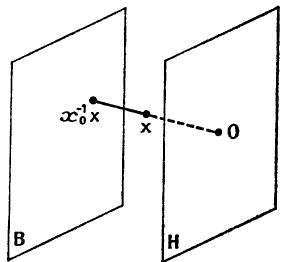
\includegraphics[keepaspectratio]{images/part001_d597a17f.jpg}}\\
Figure 4.

PROPOSITION 5. In a projective space \(\mathbf{P}_n\) ( \(n \geqslant 0\) ), the complement of a projective hyperplane H is homeomorphic to \(\mathbf{R}^n\) .

By making a projective linear transformation we may assume that H is the hyperplane whose equation is \(x_{0}=0\) . The set A of points \(\boldsymbol{x}=(x_{i})\) of \(R_{n+1}^{*}\) such that \(x_{0}\neq0\) is open and saturated with respect to \(\Delta_{n}\) ; its canonical image C in \(P_{n}\) , which is the complement of H in \(P_{n}\) , is therefore homeomorphic to the quotient of A by the equivalence relation \(\Theta\) induced on A by \(\Delta_{n}\) (Lemma 1). Let B be the hyperplane whose equation is \(x_{0}=1\) in \(R^{n+1}\) . To each point \(x\in A\) let correspond the point \(x_{0}^{-1}x\) where the line through o and x cuts B (Fig. 4); in this way we define a continuous mapping g of A onto B such that \(g(x)\) is the only point of B congruent to x modulo \(\Theta\) . It follows that B is homeomorphic to A/ \(\Theta\) (Lemma 2), hence to C; since B is homeomorphic to \(R^{n}\) , the proof is complete.

COROLLARY. Every point of \(P_{n}\) has an open neighbourhood homeomorphic to \(R^{n}\) . It follows in particular that the real projective spaces are locally connected (this follows also from Chapter I, § 11, no. 6, Proposition 12).

